\documentclass[11pt,a4paper]{article}
\usepackage[T1]{fontenc}
\usepackage{lmodern}
\usepackage[margin=1in]{geometry}
\usepackage{amsmath,amssymb,amsthm,booktabs,graphicx,array}
\usepackage{microtype}
\usepackage{xurl}
\usepackage[round,authoryear]{natbib}
\usepackage{xcolor}
\usepackage[colorlinks=true,linkcolor=blue!45!black,citecolor=blue!45!black,urlcolor=blue!45!black]{hyperref}
\usepackage{caption}
\captionsetup{font=small,labelfont=bf}
\usepackage{enumitem}
\setlength{\parskip}{3pt}
\setlength{\parindent}{1.2em}
\setlength{\emergencystretch}{2em}
\widowpenalty=10000
\clubpenalty=10000
\displaywidowpenalty=10000
\hypersetup{pdftitle={When Portfolio Maps Go Stale: Offshore Restatement and Measured External Adjustment},pdfauthor={Shivam Gupta},pdfsubject={External portfolio exposure measurement},pdfkeywords={external adjustment, nationality restatement, offshore issuance, fragmentation}}
\linespread{1.07}
\newtheorem{proposition}{Proposition}
\newtheorem{example}{Example}
\newcommand{\TV}{\operatorname{TV}}
\newcommand{\E}{\mathbb{E}}
\newcommand{\ind}{\mathbf{1}}
\newcommand{\R}{\mathcal{R}}
\newcommand{\note}[1]{\par\vspace{2pt}{\footnotesize\noindent\textit{Notes:} #1\par}}
\title{When Portfolio Maps Go Stale:\\Offshore Restatement and Measured External Adjustment}
\author{Shivam Gupta\\\small Independent Researcher, India\\\small\href{mailto:shivam1720406@gmail.com}{shivam1720406@gmail.com}}
\date{16 October 2026}
\begin{document}
\maketitle
\begin{abstract}
Nationality restatements reveal external exposures hidden by offshore issuance, but their use beyond the last mapped year introduces a second measurement problem: a current residence-based position is combined with an old, value-weighted composition of underlying issuers. We evaluate this practice using annual public restatement matrices and external portfolio positions for 2007--2020. Across eleven three-year comparisons, a stale map produces a mean total-variation distance of 3.12 percentage points in U.S. common-equity nationality shares and 6.46 points in corporate bonds, compared with 0.26 points in government bonds. The implications for measured adjustment are selective. No three-year comparison reverses the direction of China's common-equity exposure change, whereas four reverse China's corporate-bond change and seven reverse Russia's; four and three, respectively, remain when both changes must exceed 0.1 percentage point. We derive an exact accounting decomposition, sharp exposure intervals conditional on row-level drift restrictions, and a criterion for prioritizing map updates. In a historical information-acquisition experiment, updating five rows selected using earlier instability reduces common-equity error from 2.79 to 1.48 points. Results survive support restrictions and alternative portfolio treatments. The contribution is a reproducible temporal validation of nationality-restated exposures and a practical framework for maintaining them, rather than a causal estimate of fragmentation or an extrapolation to post-2022 portfolios.
\end{abstract}
\vspace{3pt}
\noindent\textbf{Keywords:} external adjustment; portfolio investment; offshore issuance; nationality restatement; geoeconomic fragmentation; financial statistics.\\
\noindent\textbf{JEL:} F21, F32, F36, G15, C81.\\
\noindent\textbf{Code and replication:} \url{https://github.com/shi1720/offshore-map-expiry}

\section{Introduction}
A statistical agency observes how much a country's investors hold in securities issued from the Cayman Islands. An analyst wants to know how much of that position represents exposure to Chinese firms. A security-level nationality mapping supplies the missing composition. If that mapping is old, however, observing the current Cayman position does not reveal its current underlying allocation. An increase in one offshore total can coexist with a decrease in one of its constituent national exposures. Updating the position while holding its composition fixed can therefore change the measured direction of external adjustment.

This is a practical issue in the infrastructure of international macroeconomic research. Nationality restatement has made it possible to study the economic links concealed by multinational financing structures. The matrices developed by \citet{cmns} are investor-, asset-, and year-specific. The original study explicitly documents changes in their entries over time. Subsequent applications must sometimes extend available mappings to years outside their coverage. For example, the data appendix of \citet{dollar} extends 2007--2017 mappings to 2002--2019 using constant offshore shares outside the mapped period. \citet[Annex 3.1, p.~89]{esm} applies a 2021 matrix to 2022--2023 portfolio positions. These are transparent and understandable responses to limited data. Their quantitative consequences deserve direct evaluation.

The question is not whether legal residence and economic nationality differ. It is how quickly a \emph{correction for that difference} becomes unreliable for a particular measurement task. The age of a mapping is only one determinant. Its effect also depends on the current importance of the residence routes whose compositions changed, the target nationality, and whether errors from different routes offset. A mapping can preserve an aggregate exposure measure while misallocating its components, or generate a large error for one asset class while remaining relatively accurate for another.

We study this problem in the December 2022 public release of the Global Capital Allocation Project (GCAP), containing annual mappings and portfolio estimates for 2007--2020. The principal application is U.S. common equity, where the asset definition avoids the mixture of common stocks and fund shares in the Coordinated Portfolio Investment Survey (CPIS). Three additional U.S. asset classes and seven non-U.S. bond books provide extensions. We hold the current residence-based book fixed and replace its current mapping with the same investor's mapping from one, two, three, or five years earlier. The contemporaneous mapping is an estimated benchmark from the same release. We refer to deviations from that benchmark as \emph{staleness errors}; they are not estimates of deviations from an unobserved true portfolio.

Three findings emerge. First, error is economically material and heterogeneous. Mean three-year total-variation (TV) distance is 3.12 percentage points for common equity, 6.46 for corporate bonds, and 14.92 for asset-backed securities, but 0.26 for government bonds. For common equity, the corresponding mean dollar amount that would have to be reassigned across nationality bins is approximately \$182.8 billion. This is a classification amount, not a loss, transaction, or capital outflow.

Second, consequences for measured adjustment are target-specific. Across the eleven three-year comparisons, a stale mapping never reverses China's common-equity trend. In corporate bonds, it reverses China's trend in four cases and Russia's in seven. The latter count falls to three when each of the two compared changes must exceed 0.1 percentage point in absolute value. For 2012--2015, Russia's corporate-bond share falls by 1.56 points under the contemporaneous maps but rises by 1.16 points when the 2012 map is held fixed. This demonstrates a measurement failure in a specified historical book; it does not identify the cause of its adjustment.

Third, the problem can be reduced without rebuilding every row. We rank residence routes by current portfolio weight multiplied by their mean annual mapping instability over the latest three available historical transitions. In the eight three-year common-equity evaluations with this history, refreshing five rows lowers mean TV distance from 2.79 to 1.48 points, a 46.95\% reduction. The same number of updates ranked by current holdings lowers it to 1.66 points. The instability rule beats holdings ranking in seven of these eight cases and in 67 of 88 country--asset--year cases overall. It does not dominate in every book.

The paper makes a bounded contribution. It provides a temporal-validation benchmark for a consequential measurement input, documents the resulting exposure and direction errors, and connects a transparent update policy to conditional exposure bounds. The accounting identities, TV inequalities, and two-factor decomposition use established mathematics. We do not claim a new theory of fragmentation, a new nationality-restatement method, or a universally optimal refresh policy. The distinctive object is the maintenance of a nationality-restatement map after its original observation date.

\section{Relation to the literature}
The residence, nationality, and currency dimensions of international balance sheets are conceptually distinct. \citet{triple} explains why treating them as coincident can obscure financial linkages. \citet{bbc} uses U.S. security-level holdings to distinguish residence-based positions from nationality-based exposures, including the role of foreign financing subsidiaries and investment funds. \citet{cmns} supplies public investor-specific matrices for restating bilateral portfolios. These contributions establish the measurement infrastructure on which our analysis depends. The temporal variation in the underlying matrices is already recognized; our question concerns the error from failing to update them.

Recent work goes beyond reassigning the issuer. \citet{beck} jointly addresses ultimate issuer nationality and the ownership of funds intermediated through euro-area financial centers. This distinction matters here: updating an issuer-side map does not resolve investor-side fund intermediation. Our non-U.S. extensions remain books attributed to the source investor under the older GCAP methodology. They should not be interpreted as a reconstruction of ultimate household ownership. The broader literature surveyed by \citet{review} similarly motivates treating different exposure concepts as answers to different economic questions.

The problem also intersects with research on external adjustment. \citet{gr} distinguishes trade and valuation channels in the dynamics of external positions. \citet{portfolio} embeds international portfolios in an analysis of global imbalances. Our decomposition has a more limited purpose: separating changes in residence weights from changes in the within-residence nationality map. Neither term is a transaction measure. Prices, purchases, corporate events, sample coverage, and classification revisions can affect the map. Consequently, the paper does not label a mapping residual as active decoupling.

Fragmentation measurement introduces additional choices. \citet{airaudo} shows that conclusions about financial portfolio fragmentation are sensitive to how geopolitical distance is constructed. We hold the country query explicit: mainland China, Russia, their union, and China plus Hong Kong. These sets avoid estimating an additional political-alignment variable. They are not proposed as a comprehensive partition of the world into geopolitical blocs. Our results isolate an accounting input that precedes the choice of a gravity specification or an alignment measure.

Finally, the symmetric decomposition below is the two-factor application of the standard Shapley approach discussed by \citet{shorrocks}. The conditional interval and refresh results follow from elementary properties of probability vectors and separable uncertainty sets. Their value in this application is operational: they identify the information needed to support a directional statement and show which mapping rows deserve attention under a declared uncertainty model. A literature search covering these strands found no study implementing this particular historical staleness and selective-refresh experiment. That search supports a narrow contribution claim; it cannot establish absolute novelty across all unpublished work.

\section{Measurement framework}
\subsection{A dated map applied to a current book}
Fix an investor and asset class, suppressing those indices. Let $x_{dt}\geq0$ be the market value of securities in the external-residence book issued from residence $d$ at date $t$. Write $X_t=\sum_d x_{dt}$ and $w_{dt}=x_{dt}/X_t$. A row-stochastic matrix $M_t$ assigns residence $d$ to nationality $k$:
\begin{equation}
 M_{dk,t}\geq0,\qquad \sum_k M_{dk,t}=1,\qquad
 p_{kt}=\sum_d w_{dt}M_{dk,t}.
 \label{eq:map}
\end{equation}
This is the mapping operation underlying the public restatement approach. We preserve the external-residence denominator even when a foreign-issued security is mapped back to the investor's own nationality. Otherwise, changing the classification would also change the denominator and complicate the interpretation of staleness.

For $s<t$, a frozen-map estimate and its error are
\begin{equation}
 \widehat p_{t|s}=w_t^{\prime}M_s,\qquad
 e_{t|s}=\widehat p_{t|s}-p_t=w_t^{\prime}(M_s-M_t).
 \label{eq:error}
\end{equation}
Vectors $w_t$ are regarded as column vectors; displayed products such as $w_t^{\prime}M_t$ are row vectors. For a target set $B$, let $b$ be its indicator vector, $z_t=p_tb$, and $\widehat z_{t|s}=\widehat p_{t|s}b$. The true and frozen \emph{benchmark-relative} changes from date $s$ are
\begin{equation}
 \Delta z=z_t-z_s,\qquad
 \widehat{\Delta z}=\widehat z_{t|s}-z_s.
 \label{eq:changes}
\end{equation}
A sign reversal occurs when their product is negative. We additionally report a material reversal requiring $|\Delta z|\geq0.001$ and $|\widehat{\Delta z}|\geq0.001$, so that changes smaller than 0.1 percentage point do not drive the substantive count.

\subsection{Why stable corporate labels do not imply a stable map}
A map entry is a value share, not merely a corporate label. Consider a residence row containing two nationality groups. Even if the identities of all securities and their holdings quantities remain fixed, differential price changes alter their value shares.

\begin{proposition}[Passive valuation]
Suppose a residence row has initial target share $a\in(0,1)$, fixed holdings quantities, and fixed nationality assignments. If each security's cumulative gross price factor lies in $[L,U]$, with $0<L\leq U$, its later target share $a'$ satisfies
\begin{equation}
 \frac{La}{La+U(1-a)}\leq a'\leq
 \frac{Ua}{Ua+L(1-a)}.
 \label{eq:prices}
\end{equation}
Both bounds are attainable under the stated restrictions.
\end{proposition}
\begin{proof}
Let the initial target and complement values be $A$ and $C$. Their later values lie in $[LA,UA]$ and $[LC,UC]$. The ratio $A'/(A'+C')$ increases in $A'$ and decreases in $C'$. Substituting the corresponding endpoints gives the bounds; applying $L$ to every security in one group and $U$ to every security in the other attains them.
\end{proof}

For example, an initial half-and-half row becomes two-thirds target exposure when target prices double while complement prices remain unchanged. Observing the new total residence value does not supply that composition. This example is purely analytical. In the empirical data, mapping changes also incorporate purchases, sales, corporate events, and changes in the underlying fund sample. We cannot separate those channels with the released aggregate matrices.

\subsection{An exact decomposition of measured adjustment}
For two dates, an exact symmetric decomposition of nationality-share changes is
\begin{align}
 p_t-p_s
 &= (w_t-w_s)^{\prime}\frac{M_t+M_s}{2}
  +\frac{(w_t+w_s)^{\prime}}{2}(M_t-M_s) \\
 &\equiv D^{w}_{s,t}+D^{M}_{s,t}.
 \label{eq:decomp}
\end{align}
The first term changes residence weights at the average mapping. The second changes the mapping at the average residence weights. Expanding the products verifies the identity; averaging the two possible update orders gives the Shapley interpretation. Multiplying by $b$ yields the decomposition for any target set.

The map component is not a residual estimate of transactions hidden offshore. A valuation shock can move both components: it can change a residence route's importance in the whole book and its composition within that route. Figure~\ref{fig:decomp} therefore uses accounting labels rather than behavioral ones. Chaining annual decompositions provides an exact decomposition of the sum of annual changes, but its allocation across components need not equal the decomposition calculated directly between the two endpoints.

\subsection{Error bounds and directional claims}
For probability vectors, $\TV(u,v)=\frac12\sum_k|u_k-v_k|$. Define row drift $\delta_d=\TV(M_{d\cdot,s},M_{d\cdot,t})$. The triangle inequality gives
\begin{equation}
 \TV(\widehat p_{t|s},p_t)\leq
 \sum_d w_{dt}\delta_d\equiv A_{t|s}.
 \label{eq:envelope}
\end{equation}
The right-hand side is an additive envelope. It can be much larger than the realized aggregate error when route errors offset. For every target set $B$, $|\widehat z_{t|s}-z_t|\leq A_{t|s}$. If a decision maker has a justified upper bound $\overline A$ and $|\widehat{\Delta z}|>\overline A$, the sign of the adjustment is preserved. The realized $A_{t|s}$ is observable only after the new map becomes available. Its historical value does not automatically provide a bound for a future crisis.

A tighter statement is possible when restrictions are supplied row by row. Let $a_d=M_{d\cdot,s}b$ and suppose the unknown current row belongs to a TV ball of radius $r_d\in[0,1]$ around its old row.

\begin{proposition}[Conditional exposure interval]
For a nonempty proper target set $B$, independent row restrictions $\TV(M_{d\cdot,t},M_{d\cdot,s})\leq r_d$ imply the sharp interval
\begin{equation}
 \underline z=\sum_d w_{dt}\max\{0,a_d-r_d\},\qquad
 \overline z=\sum_d w_{dt}\min\{1,a_d+r_d\}.
 \label{eq:interval}
\end{equation}
Its sharpness is relative to nonnegative, row-stochastic maps with no additional cross-row or nationality-total constraints.
\end{proposition}
\begin{proof}
Moving probability mass $q$ from the complement of $B$ into $B$ costs TV distance $q$, and increases the target share by $q$. Thus the largest possible target share is $\min\{1,a_d+r_d\}$; the smallest is $\max\{0,a_d-r_d\}$. Available mass in each group suffices to attain the relevant endpoint. Because each row can be chosen independently and the weights are nonnegative, the weighted endpoints are jointly attainable. Convexity fills the interval between them.
\end{proof}

Equation~\eqref{eq:interval} is a conditional sensitivity result, not a confidence interval. It makes the substantive assumption visible. Restricting feasible nationalities, imposing known issuer totals, or modeling correlated mapping revisions can narrow the set, but requires additional evidence. The replication package includes an executable interval calculation and checks the formula against a separate linear-programming formulation.

\section{Data and experimental design}
\subsection{Public release and portfolio definitions}
We use the GCAP restatement matrices, version 1.5, and bilateral external portfolios, version 1.8, both labeled December 2022 \citep{mapsdoc,positionsdoc}. The downloaded files contain 4,122,880 matrix records across all methodologies and 398,332 portfolio records. We use the \emph{Fund Holdings} nationality matrices for the principal benchmark. Matrices derived from issuance and enhanced fund holdings enter comparisons. Sales-based maps answer a different exposure question and do not enter the main experiment.

The primary book is U.S. common equity. The additional U.S. classes are corporate bonds excluding asset-backed securities, government/agency/municipal bonds, and asset-backed securities. The seven non-U.S. books contain all bonds held by Canada, Switzerland, Denmark, the euro area, the United Kingdom, Norway, and Sweden. Each book has fourteen annual observations, for a total of 154 investor--asset--year books. Australia is excluded because its published positions have a different reporting span. Non-U.S. equity is excluded because CPIS mixes fund shares and common equity and the source applies additional common-equity adjustments.

For a country investor, we exclude securities issued in that same residence. For the euro-area investor, we exclude issuers in the fixed set of nineteen euro-area members at end-2020. This convention defines an extra-area residence book throughout the sample; it is not a time-varying currency-membership experiment. Nationality reallocation can return part of any book to its home nationality, which we retain in both numerator support and denominator. The euro-area extension does not reproduce the newer joint issuer-and-fund-unwind estimates of \citet{beck}.

The source files use sparse matrices: omitted cells are zero. Where an entire residence row is absent, we use the residence identity row and record the affected current book weight. Across the comparisons, the largest unmapped fraction is 0.0691\%, in the Swedish bond book; it is 0.0099\% for U.S. common equity. Renormalizing the explicit source rows removes binary32 roundoff no larger than $5.97\times10^{-8}$ in their sums.

The released positions also contain some negative cells. We found 61 such external-book cells in the selected panel. Since the principal distance interpretation requires nonnegative weights, the baseline sets these cells to zero before normalizing. The largest removed negative mass is 0.3392\% of a signed book total, in the United Kingdom. U.S. common equity has no negative cells. We retain the signed-position version as a sensitivity calculation rather than silently treating the adjustment as immaterial.

These are revised historical estimates, not a collection of historical publication vintages. The source documentation reports interpolation and extrapolation of some missing bilateral positions. The matrices themselves are estimated from the covered fund holdings, not a census of every underlying macroeconomic claim. Consequently, the experiment isolates the consequences of using older \emph{estimated compositions within this release}; it cannot measure a real-time analyst's complete information error.

\subsection{Historical staleness experiment}
For each book, target date $t$, and horizon $h\in\{1,2,3,5\}$, we compare $w_t^{\prime}M_{t-h}$ with $w_t^{\prime}M_t$. There are 13, 12, 11, and 9 comparisons per book, respectively: 495 frozen-map comparisons across eleven books. We report means, medians, and maxima over available dates. Each date receives equal weight within its book; country books are not pooled into an artificial global representative portfolio.

TV distance measures the minimum share of the book that must be reassigned across nationality bins to reconcile two distributions. It is also the maximum absolute exposure-share error over unrestricted subsets of nationality bins. The maximizing subset is selected after seeing the error vector, so TV should not be interpreted as the error for an independently specified geopolitical bloc. For that reason, we separately report the predeclared China and Russia queries and their two unions.

The comparator maps use information dated no later than $s=t-h$: the latest investor map; the equally weighted mean of that investor's latest three maps; the equally weighted mean of other available investors' latest maps for that asset class; and the latest issuance map where available. For the U.S. common-equity comparison, the common calendar is 2012--2020, giving nine evaluations at the three-year horizon. No future-year map enters a comparator. Because the source release contains revised histories, this chronological restriction is weaker than a genuine real-time vintage restriction.

\subsection{Validation and uncertainty}
An independently implemented sparse dictionary projection reproduces all 495 TV distances and 1,980 target errors to within $5\times10^{-13}$ in shares. The largest saved symmetric-decomposition residual is below $7.1\times10^{-14}$. A separate suite contains 385 passing tests, including random accounting identities, passive-price bounds, cancellation examples, and 80 interval instances checked against linear programs. These checks establish computational agreement under the specified definitions, not the accuracy of the underlying source estimates.

For the 140 non-euro-area book--year observations, we also compare the contemporaneous reconstruction with the source's published ex-domestic restatement after removing its preserved domestic balance. The maximum country discrepancy for U.S. common equity is \$0.052 million, consistent with source precision. Some bond books differ more because the nonnegative treatment changes source cells and because of residual source conventions. We retain the full reconciliation table. An additional comparison uses the independently constructed U.S. common-stock estimates of \citet{bbc}, updated through 2024; Appendix~\ref{app:independent} reports the resulting differences rather than treating either estimate as truth.

The principal results are descriptive functions of a fixed public release. Overlapping horizons, shared country exposures, and common market events rule out treating the 495 comparisons as independent draws. We therefore do not attach conventional cross-sectional standard errors or claim causal significance. Sampling uncertainty in the underlying fund-based maps is not recoverable from these aggregate files. The results answer a finite historical measurement question, supported by explicit sensitivity checks.

\section{How large is the error from an old map?}
\subsection{Map age and asset composition}
Table~\ref{tab:age} reports the complete U.S. age profiles. Common-equity mean error rises from 1.59 points after one year to 4.19 after five years. Corporate-bond error rises from 3.52 to 8.27 points, and asset-backed error from 8.70 to 18.00. Government bonds have smaller errors at every reported horizon. These means compare different sets of origin--target dates as the horizon changes, so they are not estimates of a structural annual depreciation rate for data quality.

\begin{table}[tb]
\centering\small
\caption{U.S. nationality-share error from stale maps (percentage points)}\label{tab:age}
\begin{tabular}{lrrrrr}
\toprule
Asset class & Age & N & Mean & Median & Maximum \\
\midrule
Common equity & 1 & 13 & 1.59 & 1.50 & 2.52 \\
 & 2 & 12 & 2.45 & 2.14 & 4.03 \\
 & 3 & 11 & 3.12 & 2.93 & 5.18 \\
 & 5 & 9 & 4.19 & 3.75 & 7.18 \\
Corporate bonds & 1 & 13 & 3.52 & 3.11 & 6.18 \\
 & 2 & 12 & 5.19 & 4.69 & 8.63 \\
 & 3 & 11 & 6.46 & 6.33 & 11.31 \\
 & 5 & 9 & 8.26 & 8.37 & 11.21 \\
Government bonds & 1 & 13 & 0.12 & 0.11 & 0.29 \\
 & 2 & 12 & 0.19 & 0.15 & 0.50 \\
 & 3 & 11 & 0.26 & 0.16 & 0.66 \\
 & 5 & 9 & 0.37 & 0.32 & 0.77 \\
Asset-backed securities & 1 & 13 & 8.70 & 6.45 & 23.10 \\
 & 2 & 12 & 12.77 & 8.92 & 36.15 \\
 & 3 & 11 & 14.92 & 11.05 & 38.29 \\
 & 5 & 9 & 18.00 & 15.48 & 31.89 \\
\bottomrule
\end{tabular}

\note{TV distance between the current and frozen-map nationality shares of the same current external-residence book. Available target years are 2008--2020, 2009--2020, 2010--2020, and 2012--2020 at ages 1, 2, 3, and 5. Government includes sovereign, agency, and municipal bonds. Source: calculations from GCAP.}
\end{table}

\begin{figure}[tb]
\centering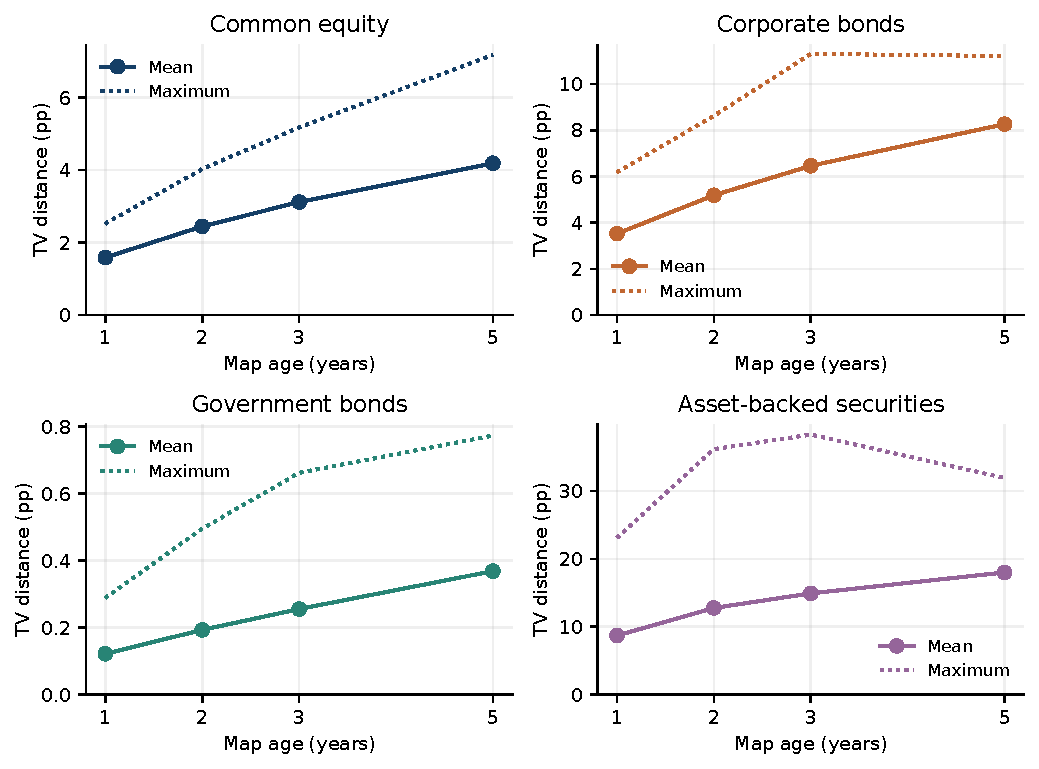
\includegraphics[width=\textwidth]{../figures/age_errors.pdf}
\caption{Error increases with map age on average, with substantial asset-class differences.}\label{fig:age}
\note{The panels deliberately have different vertical scales. Solid lines show the mean and dotted lines the maximum over the comparisons in Table~\ref{tab:age}; no confidence interpretation is assigned.}
\end{figure}

The distinction between sovereign and corporate issuance supplies an economically interpretable comparison. A nationality reassignment of a government security generally has less scope to change its issuer country than a reassignment of corporate or structured securities. This does not make the government series a causal placebo: its composition, coverage, and underlying assets differ. It shows that age alone is insufficient to characterize the loss of information. In particular, a single rule for the admissible age of every external-portfolio map would ignore the large cross-asset heterogeneity in Figure~\ref{fig:age}.

The maxima matter as well. The largest three-year common-equity error is 5.18 points, compared with a mean of 3.12. For asset-backed securities the maximum is 38.29 points. These are observed outcomes in the historical release, not tail-probability estimates. A reader interested in a particular national shock should use the target errors rather than interpret the all-destination TV maximum as a forecasted loss.

\subsection{Country-specific adjustment and sign reversals}
Table~\ref{tab:reversal} separates China and Russia. For common equity, a three-year-old map produces mean absolute China-share error of about 0.37 point but no sign reversal. Russia has two common-equity reversals, both involving at least one change smaller than 0.1 point. The stronger directional result occurs in corporate bonds. Four of eleven China comparisons reverse direction and all four meet the materiality rule; seven Russia comparisons reverse, of which three meet that rule.

\begin{table}[tb]
\centering\small
\caption{Three-year country-exposure errors and direction reversals}\label{tab:reversal}
\begin{tabular}{lrrrrr}
\toprule
Asset class & Target & N & Any reversal & Material & Mean abs. error \\
\midrule
Common equity & China & 11 & 0 & 0 & 0.37 \\
 & Russia & 11 & 2 & 0 & 0.10 \\
Corporate bonds & China & 11 & 4 & 4 & 0.73 \\
 & Russia & 11 & 7 & 3 & 0.82 \\
Government bonds & China & 11 & 0 & 0 & 0.01 \\
 & Russia & 11 & 0 & 0 & 0.00 \\
Asset-backed securities & China & 11 & 2 & 0 & 0.31 \\
 & Russia & 11 & 5 & 1 & 0.05 \\
\bottomrule
\end{tabular}

\note{A reversal compares $z_t-z_s$ with $\widehat z_{t|s}-z_s$ using the current benchmark at the origin in both cases. A material reversal requires both changes to have absolute magnitude at least 0.1 percentage point. The last column is the mean absolute level error in percentage points of the external-residence book.}
\end{table}

Figure~\ref{fig:examples} contrasts two examples. For China's common-equity share, using a 2017 map preserves the subsequent increase through 2020 but overstates its endpoint. For Russia's corporate-bond share, holding the 2012 map fixed produces the opposite direction through 2015. Its benchmark share changes from 2.51\% to 0.95\%, while the frozen-map endpoint is 3.67\%. The stale endpoint exceeds the benchmark by 2.72 percentage points. Both calculations observe the same current residence book; only the map differs.

\begin{figure}[tb]
\centering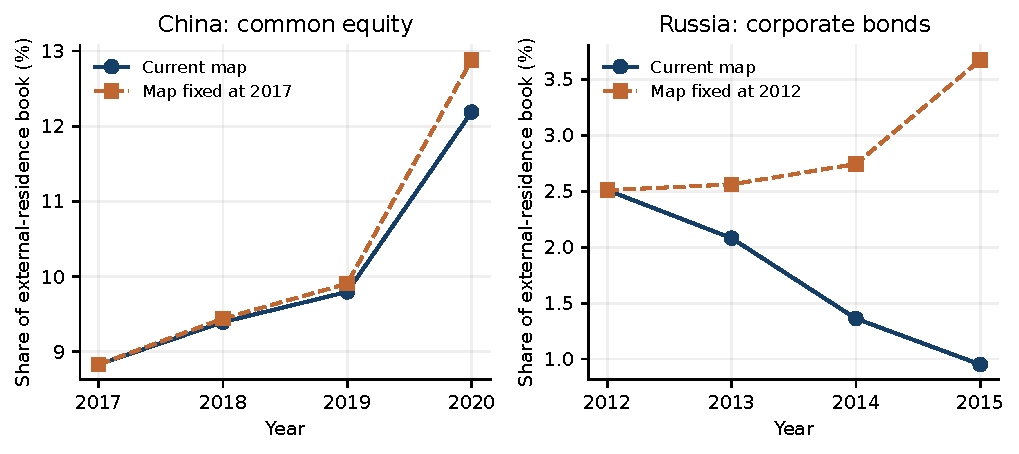
\includegraphics[width=\textwidth]{../figures/country_examples.pdf}
\caption{A stale map can preserve one trend while reversing another.}\label{fig:examples}
\note{Left: maps frozen at 2017 for U.S. common-equity exposure to mainland China. Right: maps frozen at 2012 for U.S. corporate-bond exposure to Russia. Each comparison uses the external-residence denominator for that year. These are illustrative cases selected from the full reported panel, not estimates of a policy effect.}
\end{figure}

It would be incorrect to infer that a specific sanction, change in risk appetite, or financing decision caused the right panel. The maps combine covered fund positions and classifications, and the macro book is separately measured. The valid conclusion is narrower and consequential: in this historical input, a fixed mapping can support an increase in exposure while the updated mapping supports a decrease. Conversely, the absence of a China common-equity reversal is an informative negative result. A concern about stale maps does not invalidate every measured adjustment.

Figure~\ref{fig:decomp} separates annual residence-weight and mapping contributions. The two components can reinforce each other or offset. Their relationship also explains why the largest route in the current book need not be the most valuable route to remap: a large but stable row contributes little staleness error, whereas a smaller row with rapidly changing composition can matter substantially.

\begin{figure}[tb]
\centering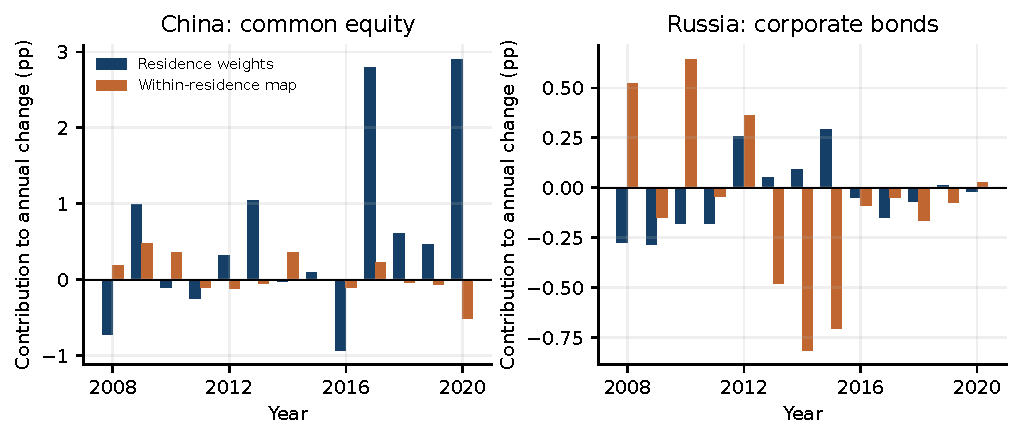
\includegraphics[width=\textwidth]{../figures/decomposition.pdf}
\caption{Residence weights and within-residence composition contribute differently to measured adjustment.}\label{fig:decomp}
\note{Annual symmetric decomposition in equation~\eqref{eq:decomp}. Bars show percentage-point contributions, which sum within each year to the actual benchmark share change. Neither component identifies net purchases or a causal geopolitical response.}
\end{figure}

\subsection{Which residence routes matter?}
For each comparison, the contribution of residence $d$ to the additive envelope is $w_{dt}\delta_d$. Figure~\ref{fig:routes} averages this quantity over the three-year U.S. comparisons. It does not average signed target errors. In common equity, the United Kingdom is the largest contributor to this envelope, followed by Ireland and the Cayman Islands. Non-haven residence rows matter because the main experiment uses full nationality restatement. Restricting attention to only a few conventional offshore centers can therefore miss part of the maintenance problem.

\begin{figure}[tb]
\centering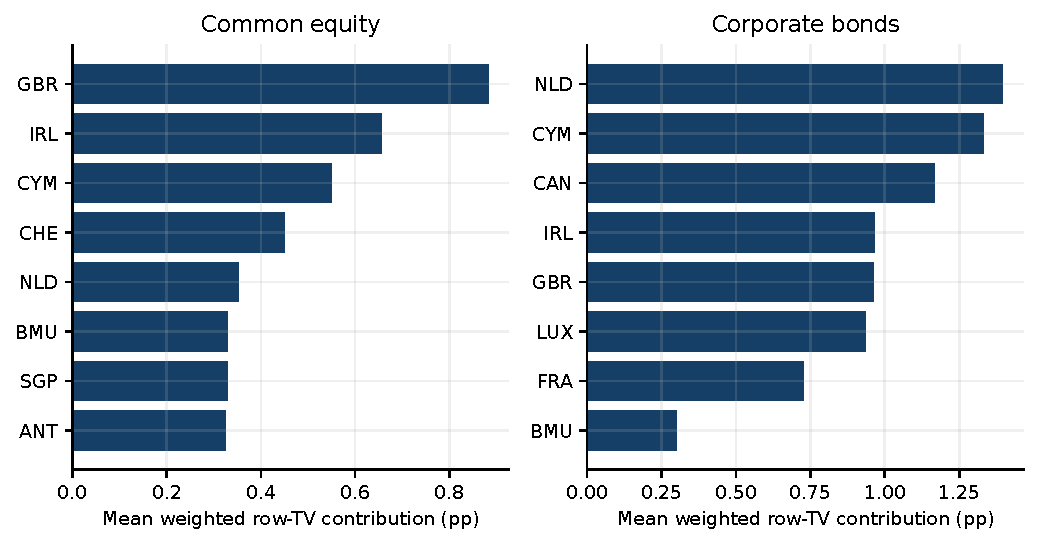
\includegraphics[width=\textwidth]{../figures/route_contributions.pdf}
\caption{A small set of residence routes accounts for substantial mapping instability.}\label{fig:routes}
\note{Eight largest residence contributions to the mean three-year additive envelope, calculated separately by asset class. ISO codes identify the residence of the immediate issuer. Contributions are nonnegative and can exceed aggregate TV error because signed destination errors cancel across routes.}
\end{figure}

This evidence supports measuring the route--composition interaction rather than counting offshore subsidiaries or using the size of a financial center alone. It also cautions against interpreting the envelope as realized exposure error. If two routes overstate and understate the same nationality by similar amounts, a current aggregate can look accurate while its underlying route attributions are wrong.

\section{Maintaining a map with a limited update budget}
\subsection{What can an exact row refresh guarantee?}
Suppose a statistical agency or data vendor can refresh selected residence rows exactly, while other rows retain their old values. Under the conditional row restrictions in Proposition~2, row $d$ contributes
\begin{equation}
 v_d=w_{dt}\left[\min\{1,a_d+r_d\}-\max\{0,a_d-r_d\}\right]
 \label{eq:value}
\end{equation}
to the width of the target-exposure interval. Observing that row eliminates its uncertainty.

\begin{proposition}[Equal-cost refresh priority]
If any $K$ rows can be observed exactly at equal cost, selecting the $K$ largest values in equation~\eqref{eq:value} minimizes the remaining width of the conditional target-exposure interval. For the additive TV envelope with row radii $r_d$, selecting the $K$ largest $w_{dt}r_d$ minimizes its remaining bound.
\end{proposition}
\begin{proof}
The unrevealed interval width is the sum of $v_d$ over the rows not observed. Replacing a selected row by an unselected row with larger $v_d$ weakly reduces that sum. Iterating this exchange gives the stated rule. The same argument applies to the additive envelope, replacing $v_d$ with $w_{dt}r_d$.
\end{proof}

The result concerns a separable uncertainty width, not realized TV distance or the monetary value of information in a general decision problem. Unequal acquisition costs produce a budgeted selection problem; cross-row restrictions destroy the simple additive ranking. In addition, partial refresh can \emph{increase} realized aggregate error by removing a favorable cancellation. For example, with weights $(1/2,1/2)$, old rows $(1,0)$ and $(0,1)$, and current rows $(0,1)$ and $(1,0)$, the old and current aggregate distributions coincide. Refreshing either single row creates a TV error of $1/2$. The replication tests include this counterexample. It explains why an update rule needs an explicit objective.

\subsection{A historical information-acquisition experiment}
The theoretical radii are not known in an operational application. We evaluate a transparent heuristic using earlier instability. At origin $s$, define
\begin{equation}
 \widehat r_{d,s}=\frac13\sum_{u=s-2}^{s}
 \TV(M_{d\cdot,u},M_{d\cdot,u-1}),\qquad
 q_{d,t|s}=w_{dt}\widehat r_{d,s}.
 \label{eq:priority}
\end{equation}
We rank all positive-current-weight residence rows by $q_{d,t|s}$ and refresh the first $K\in\{1,3,5,10\}$ with their target-date values. This assumes that a selected current row can be acquired exactly, even though the rest of the current map remains unavailable. Current residence holdings are available by construction; only mapping information is restricted to the origin. Thus this is a retrospective experiment in acquiring information \emph{at the target date}, not a forecast that knows future book weights at the origin.

The comparison uses $h=3$ and origins 2010--2017, so all three historical transitions are available. There are eight evaluations per book and 88 overall. Current-weight ranking is a strong simple comparator. Random selection draws 200 subsets at each budget and case with a fixed seed. An ex post comparator ranks rows by their realized $w_{dt}\delta_d$; this minimizes the realized additive envelope among equal-count updates, but is not an oracle for aggregate TV distance. None of the historical instability scores is claimed to be a valid future radius for Proposition~2.

Figure~\ref{fig:refresh} and Table~\ref{tab:refresh} report the outcomes. Updating five rows by historical instability lowers common-equity mean TV from 2.79 to 1.48 points. In corporate bonds it lowers mean TV from 5.71 to 3.21 points, compared with 3.94 points under current-weight ranking. In seven of eight common-equity cases, the instability rule beats the holdings rule. Across all books it wins 67 of 88 five-row comparisons. Denmark's all-bond book and U.S. asset-backed securities have lower mean errors under holdings ranking. These exceptions limit any claim of a universally superior acquisition strategy.

\begin{figure}[tb]
\centering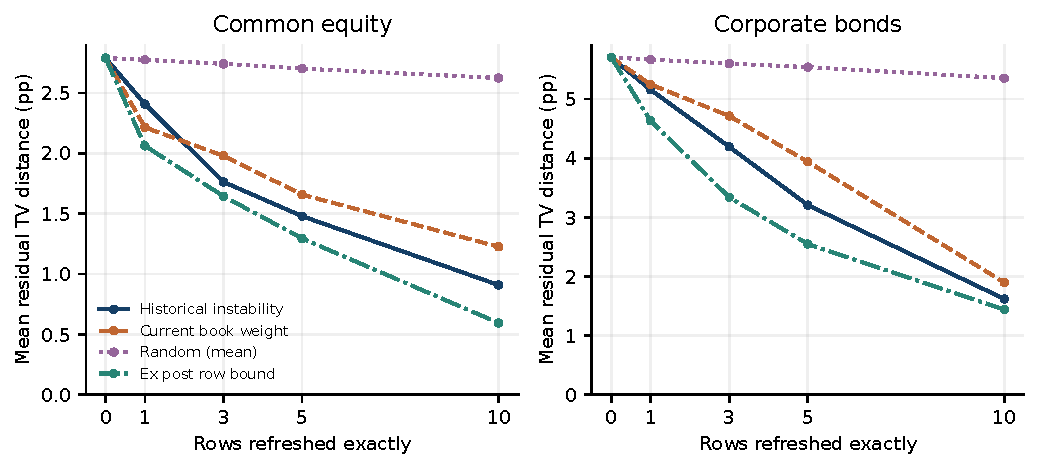
\includegraphics[width=\textwidth]{../figures/selective_refresh.pdf}
\caption{Selective refresh reduces historical mapping error without rebuilding every residence row.}\label{fig:refresh}
\note{Three-year maps; target years 2013--2020. All policies observe the same current book. ``Ex post row bound'' uses future row drift and is an infeasible reference policy, not a deployable predictor or a TV-optimal oracle. Random curves average 200 subsets per case and budget.}
\end{figure}

\begin{table}[tb]
\centering\small
\caption{Five exact row updates: mean residual TV distance (percentage points)}\label{tab:refresh}
\begin{tabular}{lrrrr}
\toprule
Book & Stale & Instability & Weight & Ex post bound \\
\midrule
U.S. equity & 2.79 & 1.48 & 1.66 & 1.29 \\
U.S. corporate & 5.71 & 3.21 & 3.94 & 2.55 \\
U.S. government & 0.30 & 0.07 & 0.16 & 0.02 \\
U.S. asset-backed & 10.86 & 0.95 & 0.79 & 0.72 \\
CAN bonds & 3.90 & 1.12 & 1.17 & 0.90 \\
CHE bonds & 4.69 & 2.14 & 3.42 & 2.00 \\
DNK bonds & 6.08 & 2.75 & 2.61 & 2.09 \\
EMU bonds & 2.73 & 0.82 & 1.17 & 0.75 \\
GBR bonds & 3.19 & 2.02 & 2.28 & 1.80 \\
NOR bonds & 3.49 & 1.91 & 2.76 & 1.62 \\
SWE bonds & 9.76 & 3.90 & 5.85 & 2.56 \\
\bottomrule
\end{tabular}

\note{Eight three-year evaluations per book, target years 2013--2020. ``Stale'' applies no updates. ``Instability'' uses equation~\eqref{eq:priority}; ``Weight'' ranks current residence weights. The final column ranks ex post contributions to the additive envelope and uses information unavailable to the historical policy.}
\end{table}

The potential operational saving is in the number of residence compositions requiring acquisition, not in a measured reduction in staff hours or vendor charges. Large routes can contain many issuers, and their costs need not be equal. Moreover, the exact row oracle overstates what a partial security-level refresh may deliver. The result nevertheless supplies a concrete policy experiment: on these historical books, the value of maintaining all rows is highly unequal, and past instability contains useful information beyond current holdings size.

\section{Alternative maps, support, and interpretation}
\subsection{Smoothing and pooling do not remove the problem}
Table~\ref{tab:predictors} compares four maps on the same nine common-equity target years. The most recent investor-specific map performs better in mean TV than the three-map average, other-investor average, or issuance map. Temporal smoothing reduces responsiveness as well as noise; a globally representative issuance composition need not represent the securities a particular country's investors hold. These results do not rule out a better forecasting model. They show that simple pooling is not an automatic remedy for age.

\begin{table}[tb]
\centering\small
\caption{Alternative dated maps for U.S. common equity, three-year horizon}\label{tab:predictors}
\begin{tabular}{lrrr}
\toprule
Map used & N & Mean TV (pp) & Maximum TV (pp) \\
\midrule
Latest investor map & 9 & 2.79 & 3.52 \\
Mean of latest three maps & 9 & 3.30 & 5.08 \\
Other-investor mean & 9 & 5.99 & 7.72 \\
Issuance map & 9 & 6.06 & 7.33 \\
\bottomrule
\end{tabular}

\note{Common target years 2012--2020. Comparator inputs have dates no later than the origin. Peer maps receive equal weight across other covered investors with that asset-class map. Issuance maps describe the investable securities distribution rather than an investor-specific portfolio.}
\end{table}

Enhanced fund-holdings maps allow an additional U.S. check. Their mean three-year common-equity staleness error is 3.15 points, compared with 3.12 using the baseline fund map. The mean gap between the two contemporaneous benchmarks over those comparisons is 0.08 point. For corporate bonds, enhanced-map staleness error is 5.28 points and the contemporaneous benchmark gap is 3.04 points. The equity finding is stable to this alternative, while the larger bond benchmark difference reinforces the need to distinguish map age from map estimation and coverage.

\subsection{Other investors and sensitivity to data conventions}
Table~\ref{tab:extensions} shows three-year all-bond errors for the seven additional investors. Means range from 3.37 points in the extra-euro-area book to 10.11 in Sweden. The Canadian maximum reaches 18.49 points, compared with its 5.24-point mean. These books differ in asset composition and source coverage, so the ordering is not a ranking of countries' statistical quality or geopolitical vulnerability. It demonstrates that the maintenance issue extends beyond the U.S. primary application.

\begin{table}[tb]
\centering\small
\caption{Three-year staleness in other investors' all-bond books}\label{tab:extensions}
\begin{tabular}{lrrrr}
\toprule
Investor & N & Mean TV (pp) & Maximum TV (pp) & Unmapped weight (\%) \\
\midrule
CAN & 11 & 5.24 & 18.49 & 0.002 \\
CHE & 11 & 4.59 & 5.62 & 0.009 \\
DNK & 11 & 5.81 & 8.20 & 0.053 \\
EMU & 11 & 3.37 & 5.49 & 0.022 \\
GBR & 11 & 3.44 & 4.71 & 0.018 \\
NOR & 11 & 3.59 & 4.08 & 0.034 \\
SWE & 11 & 10.11 & 15.29 & 0.069 \\
\bottomrule
\end{tabular}

\note{Eleven comparisons per investor, target years 2010--2020. Unmapped weight is the maximum target-book weight on residence rows absent from the old map, reported as a percentage of the book. EMU excludes the fixed end-2020 nineteen-country euro-area residence set.}
\end{table}

Retaining signed source positions changes any saved TV calculation by at most 0.039 percentage point. Restricting each old/current pair to residence routes present in both maps and renormalizing their book changes any error by at most 0.009 point. The primary U.S. common-equity findings are therefore not driven by negative positions or absent rows. These sensitivity checks alter a defined calculation; they do not validate unobserved securities outside the covered fund data.

Appendix~\ref{app:routes} further restricts restatement to sixteen financial-center residences identified by \citet{bbc}. Three-year common-equity mean error remains 1.88 points and corporate-bond error 4.34 points. Excluding the legacy Netherlands Antilles and associated successor codes yields means of 3.02 and 6.36 points, respectively. Thus the central findings are not solely an artifact of applying full-nationality corrections to non-center countries or of territorial-code changes. The center-only result is a different exposure convention; the residual difference cannot be interpreted as a clean attribution of the full TV error because cancellation changes when routes are removed.

\subsection{Implications for fragmentation research and risk measurement}
The findings suggest three reporting practices. First, every nationality-restated exposure should carry both the position date and the map date. The observation date of a current macroeconomic stock does not establish the freshness of its economic composition. Second, directional conclusions should be checked against target-specific mapping sensitivity. A small movement in a country's exposure can be less informative than a large change even when both come from the same statistical pipeline. Third, maintenance should follow exposure-weighted instability and the analytical query, with explicit recognition that monitoring an interval width and minimizing realized signed error are different objectives.

For a linear country haircut $H\in[0,1]$, the difference between two calculated losses on the same book is $HX_t|\widehat z-z|$. For an arbitrary vector of nationality haircuts in $[0,H]$, it is bounded by $HX_t\TV(\widehat p,p)$. These are accounting statements, not estimates of crisis losses. They explain why a classification error can matter commercially for exposure dashboards, scenario testing, and data procurement even when it is not itself a market loss. Existing look-through products already address exposure aggregation \citep{crd}; the proposed contribution is an explicit audit of the age and uncertainty of the map used in that aggregation. Deployment would require institution-specific coverage, acquisition costs, and appropriately licensed inputs.

The same caution applies to global imbalances. The paper studies gross assets in specified portfolio books. It does not recover complete national external balance sheets, foreign direct investment, bank claims, reserve portfolios, hedges, or the currency composition of all liabilities. An issuer-nationality map does not determine which legal entity can be sanctioned or whether its assets can be frozen. Residence remains relevant for law and regulation. Measurement should preserve these distinct concepts rather than replace one universal country label with another.

\section{Conclusion}
A current residence-based portfolio stock combined with an old nationality map is a dated-composition estimate. Historical validation shows that its error can be large, varies sharply by asset class, and can reverse particular measured exposure changes. It does not reverse every trend: China's common-equity direction is preserved in all eleven three-year comparisons, while several corporate-bond trends are not.

The empirical contribution is an auditable benchmark for this maintenance problem. The analytical contribution is a transparent connection between row drift, exposure sensitivity, directional statements, and the value of observing particular rows. A limited number of updates selected using earlier instability substantially reduces historical error, although simple holdings ranking is preferable in some books. The appropriate next step is to test these maintenance policies on genuinely dated releases and independently observed current compositions, especially across major fragmentation episodes. The historical results provide a reason to perform those checks and a reproducible method for doing so; they do not substitute for that evidence.

\paragraph{Data and code availability.}
All original analysis code, saved aggregate results, figure-generation scripts, tests, the analysis log, and the manuscript source are available at \url{https://github.com/shi1720/offshore-map-expiry}. The data downloader verifies hashes of the source files used here. Original GCAP data remain subject to the providers' academic-research and educational-use terms and are downloaded from the providers rather than redistributed. These data are based on the work in Coppola, Maggiori, Neiman and Schreger (2021) and were obtained from \url{www.globalcapitalallocation.com}. The Federal Reserve comparison uses the December 2025 update accompanying Bertaut, Bressler and Curcuru (2019). The analysis log distinguishes the initial design from later robustness extensions.

\clearpage
\begin{thebibliography}{99}
\small\raggedright
\bibitem[Airaudo et~al.(2025)]{airaudo} Airaudo, Florencia S., Fran\c{c}ois de Soyres, Keith Richards, and Ana Maria Santacreu. 2025. ``Measuring Geopolitical Fragmentation: Implications for Trade, Financial Flows, and Economic Policy.'' \textit{Federal Reserve Bank of St. Louis Review} 107(12): 1--30. \href{https://doi.org/10.20955/r.2025.12}{doi:10.20955/r.2025.12}.
\bibitem[Avdjiev et~al.(2015)]{triple} Avdjiev, Stefan, Robert N. McCauley, and Hyun Song Shin. 2015. ``Breaking Free of the Triple Coincidence in International Finance.'' BIS Working Paper 524. \url{https://www.bis.org/publ/work524.pdf}.
\bibitem[Beck et~al.(2026)]{beck} Beck, Roland, Antonio Coppola, Angus Lewis, Matteo Maggiori, Martin Schmitz, and Jesse Schreger. 2026. ``The Geography of Capital Allocation in the Euro Area.'' Working paper, February. \url{https://globalcapitalallocation.s3.us-east-2.amazonaws.com/GCAP_ECB_OOFCs.pdf}.
\bibitem[Bertaut et~al.(2019)]{bbc} Bertaut, Carol C., Beau Bressler, and Stephanie Curcuru. 2019. ``Globalization and the Geography of Capital Flows.'' \textit{FEDS Notes}, September 6. Data updated December 22, 2025, covering 2003--2024. \href{https://doi.org/10.17016/2380-7172.2446}{doi:10.17016/2380-7172.2446}.
\bibitem[Charles River Development(n.d.)]{crd} Charles River Development. n.d. ``How Fund Look-through Improves Buy-side Risk Monitoring and Performance Evaluation.'' Technical article. \url{https://www.crd.com/wp-content/uploads/2018/01/BobsGuide-CRD_FundLookthroughImprovesBuysideRiskEvaluation.pdf}.
\bibitem[Coppola et~al.(2021)]{cmns} Coppola, Antonio, Matteo Maggiori, Brent Neiman, and Jesse Schreger. 2021. ``Redrawing the Map of Global Capital Flows: The Role of Cross-Border Financing and Tax Havens.'' \textit{Quarterly Journal of Economics} 136(3): 1499--1556. \href{https://doi.org/10.1093/qje/qjab014}{doi:10.1093/qje/qjab014}.
\bibitem[Coppola et~al.(2022a)]{mapsdoc} Coppola, Antonio, Matteo Maggiori, Brent Neiman, and Jesse Schreger. 2022a. ``Restatement Matrices for Bilateral External Portfolios.'' GCAP data documentation, December, version 1.5. \url{https://globalcapitalallocation.s3.us-east-2.amazonaws.com/RestatementMatrices_ReadMe.pdf}.
\bibitem[Coppola et~al.(2022b)]{positionsdoc} Coppola, Antonio, Matteo Maggiori, Brent Neiman, and Jesse Schreger. 2022b. ``Restated Bilateral External Portfolios.'' GCAP data documentation, December, version 1.8. \url{https://globalcapitalallocation.s3.us-east-2.amazonaws.com/Restated_Bilateral_External_Portfolios_ReadMe.pdf}.
\bibitem[Florez-Orrego et~al.(2024)]{review} Florez-Orrego, Sergio, Matteo Maggiori, Jesse Schreger, Ziwen Sun, and Serdil Tinda. 2024. ``Global Capital Allocation.'' \textit{Annual Review of Economics} 16: 623--653. \href{https://doi.org/10.1146/annurev-economics-081623-020427}{doi:10.1146/annurev-economics-081623-020427}.
\bibitem[Gourinchas and Rey(2007)]{gr} Gourinchas, Pierre-Olivier, and H\'el\`ene Rey. 2007. ``International Financial Adjustment.'' \textit{Journal of Political Economy} 115(4): 665--703. \href{https://doi.org/10.1086/521966}{doi:10.1086/521966}.
\bibitem[Hudecz et~al.(2024)]{esm} Hudecz, Gergely, Alexandre Lauwers, Yasin Mimir, Graciela Schiliuk, Li Lian Ong, Hongyan Zhao, and Diana del Rosario. 2024. ``Geoeconomic Fragmentation: Implications for the Euro Area and ASEAN+3 Regions.'' ESM Discussion Paper 23, October; updated December. \url{https://www.esm.europa.eu/publications/geoeconomic-fragmentation-implications-euro-area-and-asean3-regions}.
\bibitem[Jiang et~al.(2022)]{dollar} Jiang, Zhengyang, Robert J. Richmond, and Tony Zhang. 2022. ``Understanding the Strength of the Dollar.'' International Finance Discussion Papers 1366, Board of Governors of the Federal Reserve System. \url{https://www.federalreserve.gov/econres/ifdp/files/ifdp1366.pdf}.
\bibitem[Jiang et~al.(2024)]{portfolio} Jiang, Zhengyang, Robert J. Richmond, and Tony Zhang. 2024. ``A Portfolio Approach to Global Imbalances.'' \textit{Journal of Finance} 79(3): 2025--2076. \href{https://doi.org/10.1111/jofi.13333}{doi:10.1111/jofi.13333}.
\bibitem[Shorrocks(2013)]{shorrocks} Shorrocks, Anthony F. 2013. ``Decomposition Procedures for Distributional Analysis: A Unified Framework Based on the Shapley Value.'' \textit{Journal of Economic Inequality} 11: 99--126. \href{https://doi.org/10.1007/s10888-011-9214-z}{doi:10.1007/s10888-011-9214-z}.
\end{thebibliography}

\clearpage\appendix
\section{Implementation details and mathematical checks}\label{app:implementation}
\subsection{Reconstruction algorithm}
The replication pipeline performs the following operations for each investor--asset--year book.
\begin{enumerate}[leftmargin=1.8em,itemsep=2pt]
\item Read the two pinned Stata files, retaining the asset-class and methodology labels. Reject duplicate residence--nationality cells and duplicate issuer positions.
\item Construct a common support containing all source residence, nationality, and portfolio issuer codes. There are 244 codes, including source residual and supranational categories. A missing matrix cell is zero; a missing entire row uses the identity convention and contributes to the unmapped-weight report.
\item Normalize explicit map rows to sum to one. Remove domestic residence holdings under the stated country or fixed-euro-area convention. Retain a copy of signed source positions; set negative cells to zero for the probability-book baseline.
\item Apply each dated map to the same target-date weights. Save distribution distances, target shares, signs, additive envelopes, support diagnostics, and route contributions before creating any paper table or figure.
\item In the refresh experiment, replace selected old rows by the actual current rows. Compute the resulting nationality vector directly as the old vector plus the sum of selected weighted row changes. This operation is algebraically equivalent to constructing a complete partially refreshed matrix.
\end{enumerate}
The independent verifier does not import the projection or panel-building functions. It constructs sparse row dictionaries, iterates over each position and destination, and compares the resulting distance and target errors with the saved records. Agreement between implementations protects against projection and indexing errors, while their common source files and stated book definitions remain shared assumptions.

\subsection{Loss interpretation of total variation}
Let $v=\widehat p-p$ with $\sum_kv_k=0$. For any $h_k\in[0,H]$,
\begin{equation}
 |\textstyle\sum_k h_k v_k|\leq H\sum_{k:v_k>0}v_k
 =H\TV(\widehat p,p).
\end{equation}
The bound is attained by setting $h_k=H$ on the positive support and zero elsewhere. This maximizing haircut vector depends on the realized error vector. It is a worst-case linear sensitivity, not a preselected geopolitical stress scenario.

\subsection{Signed-position sensitivity}
Suppose a source book has positive mass $P$ and negative mass $N$, with signed total $S=P-N>0$. The baseline nonnegative weights normalize positive positions by $P$, whereas the signed sensitivity normalizes all positions by $S$. The half-$\ell_1$ distance between these two input vectors is $N/S$. Row-stochastic maps contract this distance by the triangle inequality, even though the signed output is not a probability distribution. Consequently, the difference between the baseline and signed \emph{staleness distances} is at most $2N/S$. This bound is conservative; the observed maximum difference is 0.0386 percentage point. Inference about the economic meaning of a negative source position requires its reporting provenance, which these aggregate files do not resolve.

\subsection{A linear-programming check of Proposition 2}
For one row, introduce variables $q_k\geq0$ and $u_k\geq0$. The feasible set is
\begin{equation}
 \sum_kq_k=1,\quad q_k-M_{dk,s}\leq u_k,\quad
 M_{dk,s}-q_k\leq u_k,\quad\sum_ku_k\leq2r_d.
\end{equation}
Minimizing or maximizing $\sum_{k\in B}q_k$ gives the row endpoints independently of the closed-form implementation. Eighty randomized four-row, five-nationality instances compare the weighted LP optima with equation~\eqref{eq:interval}. Exhaustive two-row selection among four candidates also verifies the interval-width priority rule. These are implementation tests accompanying the proofs, not empirical evidence about plausible radii.

\section{Financial-center routes and territorial codes}\label{app:routes}
Table~\ref{tab:routesensitivity} compares the full-nationality experiment with two alternative calculations. The center-route version maps only Bermuda, the British Virgin Islands, Cayman Islands, Cura\c{c}ao, Guernsey, Ireland, Isle of Man, Jersey, Liberia, Luxembourg, the Netherlands, Malta, Marshall Islands, Mauritius, Panama, and Switzerland. This set follows the financial-center definition in \citet[footnote 13]{bbc}; it is not an estimate of a geopolitical bloc and is not identical to the GCAP tax-haven list. All other residence rows remain on the identity in both map dates.

The territorial-code sensitivity excludes ANT, BES, CUW, and SXM residence rows from the book and renormalizes the remaining weights. It avoids attributing a mechanical effect of the Netherlands Antilles' successor-code treatment to the economic persistence of a map. The resulting errors remain close to the full baseline. Neither sensitivity corrects every possible reporting or classification break.

\begin{table}[h]
\centering\small
\caption{Mean three-year error under alternative route conventions (percentage points)}\label{tab:routesensitivity}
\resizebox{\textwidth}{!}{\begin{tabular}{lrrr}
\toprule
Asset class & Full & Center routes & Territorial-code exclusion \\
\midrule
Common equity & 3.12 & 1.88 & 3.02 \\
Corporate bonds & 6.46 & 4.34 & 6.36 \\
Government bonds & 0.26 & 0.12 & 0.26 \\
Asset-backed securities & 14.92 & 13.35 & 14.92 \\
\bottomrule
\end{tabular}
}
\note{Eleven comparisons per asset class. ``Center routes'' freezes non-center rows at the residence identity in both old and current maps. ``Territorial-code exclusion'' removes the four specified residence codes before normalization. Changes in cancellation mean the full error is not the sum of center and non-center TV distances.}
\end{table}

\section{An independent U.S. common-stock benchmark}\label{app:independent}
The December 2025 update accompanying \citet{bbc} provides residence- and nationality-based U.S. holdings through 2024. These are independent authors' estimates based on security-level TIC holdings, rather than the fund-weighted restatement used in our principal experiment. They use a different assignment procedure and a later data revision. We compare their common-stock target shares using each dataset's own total external-residence common-stock book. The grand-total record supplies the denominator in the Bertaut--Bressler--Curcuru files; it is excluded from any aggregation of country observations to avoid double counting.

Table~\ref{tab:fed} makes the estimation differences visible. In 2020, their China nationality share is 11.34\%, compared with 12.19\% in the GCAP reconstruction; the corresponding Russia shares are 0.65\% and 0.81\%. This difference should not be added mechanically to a staleness error or interpreted as proof that either source is correct. It demonstrates that contemporaneous estimation and data vintage are separate from the age experiment. Their 2024 estimates further show why historical error magnitudes should not be treated as measurements of current exposures.

\begin{table}[h]
\centering\small
\caption{Independent common-equity exposure comparison (percent of each source book)}\label{tab:fed}
\begin{tabular}{lrrrr}
\toprule
Year & Target & BBC nationality & BBC residence & CMNS nationality \\
\midrule
2017 & China & 8.22 & 1.96 & 8.83 \\
2017 & Russia & 0.78 & 0.70 & 0.76 \\
2020 & China & 11.34 & 2.76 & 12.19 \\
2020 & Russia & 0.65 & 0.62 & 0.81 \\
2024 & China & 6.50 & 2.27 & -- \\
2024 & Russia & 0.16 & 0.12 & -- \\
\bottomrule
\end{tabular}

\note{BBC denotes Bertaut, Bressler and Curcuru, December 2025 data update. CMNS denotes the GCAP fund-map reconstruction. Data definitions and revisions differ. No GCAP observation after 2020 is imputed.}
\end{table}
\begin{figure}[tb]
\centering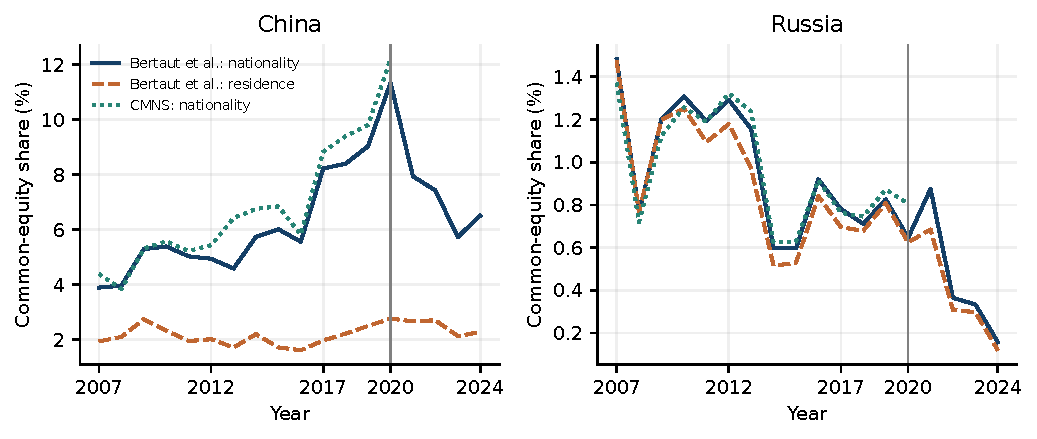
\includegraphics[width=\textwidth]{../figures/external_comparison.pdf}
\caption{Independent estimates, residence exposure, and the boundary of the historical map study.}\label{fig:fed}
\note{Each series is divided by its own external-residence common-stock total. The vertical line marks the end of the principal GCAP sample, not a structural break. Post-2020 values come solely from the updated Bertaut--Bressler--Curcuru estimates; they do not validate the GCAP frozen-map counterfactual in those years.}
\end{figure}

\section{Replication scope and research design record}
An initial analysis plan preceded exposure-error calculations; it was not externally preregistered. The repository records later extensions and reproduces every figure and table from saved results. SHA-256 hashes pin the raw inputs. Tests verify calculations under the stated definitions.
\end{document}
